\documentclass[11pt]{article}

\usepackage{graphicx}
\usepackage[top=25mm, bottom=25mm, left=25mm, right=25mm, a4paper]{geometry}
\usepackage{amsmath}
\usepackage{enumitem}
\usepackage{float}
\usepackage{fancyhdr}
\usepackage{booktabs}
\usepackage{tikz}
\usepackage{steinmetz}
\usepackage{pgfplots}
\pgfplotsset{compat=1.18}

\pagestyle{fancy}
\fancyhf{}
\fancyhead[R]{Baturay Kafkas - 2240357068 - Electrical \& Electronics Engineering}

\rfoot{\thepage}
\renewcommand{\headrulewidth}{0pt} 
\renewcommand{\footrulewidth}{0pt}
\sloppy

\begin{document}

\begin{center}
\large
\textbf{ELE214 - Electronics Laboratory I Preliminary Work 3}
\end{center}

\section{Questions}

\begin{enumerate}[leftmargin=*,label=\textbf{\arabic*.}]

\item Explain how you can test a BJT whether it is defective or not. Also propose a method to determine the type of the BJT (NPN or PNP).

\item Draw the input characteristics curve ($I_B-V_{BE}$) for a typical transistor taking three different $V_{CE}$ values. 

\item Draw the output characteristics curve ($I_C-V_{CE}$) for a typical transistor taking three different base currents. Indicate the cut-off, active, and saturation regions on the curve. 

\item Read the experimental section carefully to ensure the purpose of each step. 

\end{enumerate}

\textbf{Experimental Work (Simulation of 2-3)}

\begin{enumerate}[leftmargin=*,label=\textbf{\arabic*.}]

\item Test the BC177 transistor and determine its type.

\begin{minipage}{0.47\textwidth}
\begin{figure}[H]
    \centering
    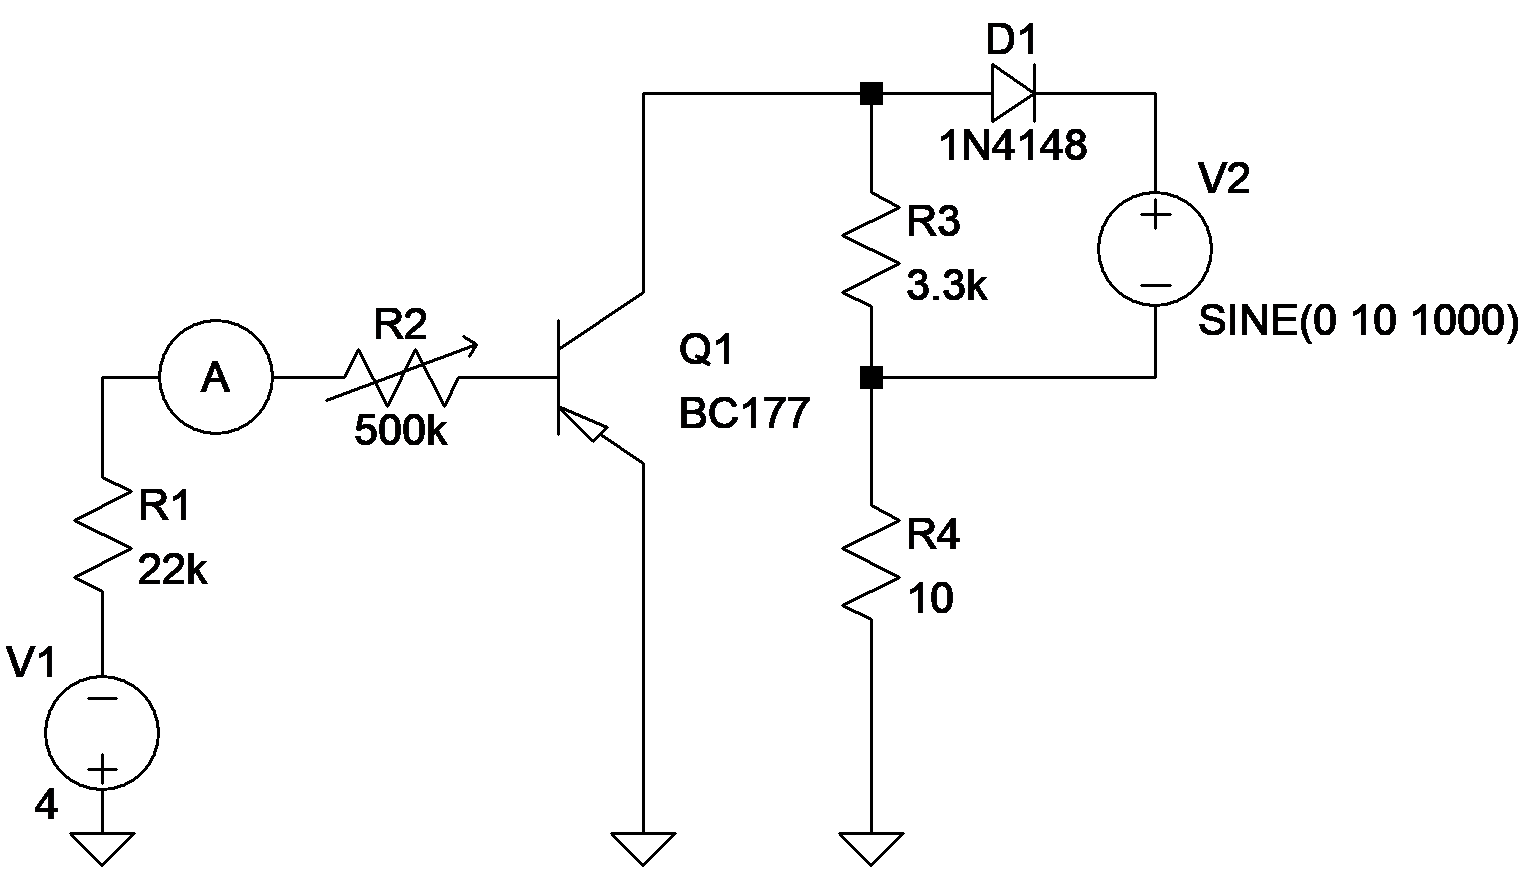
\includegraphics[width=1\linewidth]{c1.png}
    \textit{Figure 1}
\end{figure}
\end{minipage}\hfill\begin{minipage}{0.47\textwidth}
\begin{figure}[H]
    \centering
    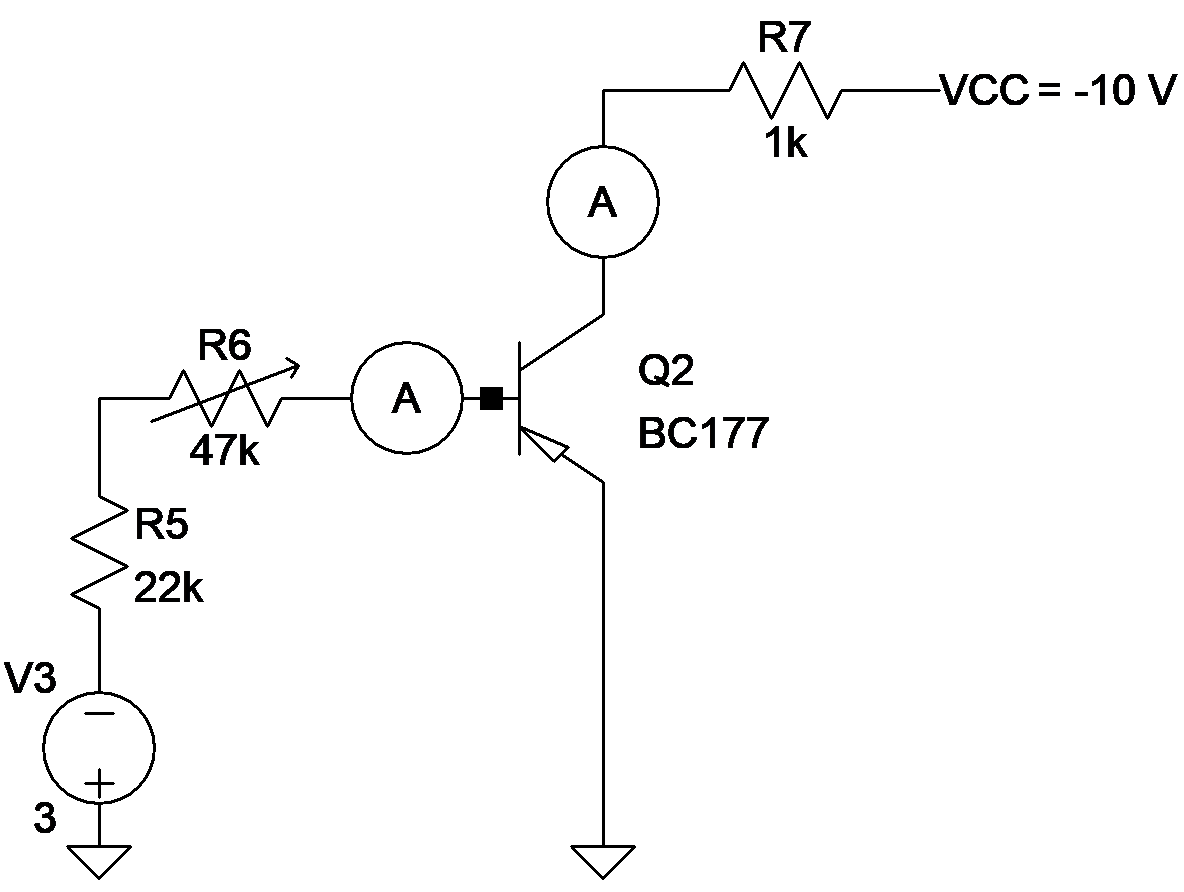
\includegraphics[width=1\linewidth]{c2.png}
    \textit{Figure 2}
\end{figure}
\end{minipage}

\item Set up the circuit in \textit{Figure 1} setting $V_s=10\sin(2\pi(1000)t)$. Observe the output characteristics on the oscilloscope for three different values of base current. Plot the results. 

\item Set up the circuit in \textit{Figure 2}. For three positions of the potentiometer (minimum, medium and maximum resistance), measure collector currents for the base currents in the previous part. Also record the base resistances for each case. 

\end{enumerate}

\section{Answers}

\begin{enumerate}[leftmargin=*,label=\textbf{\arabic*.}]

\item We can test the functionality of a BJT transistor by means of a multimeter. In order for the BJT to be healthy, there shouldn't be conduction between the collector and the emitter if the back-to-back diodes analogy is considered. If there is no conduction between any terminals, then the BJT acts as an open-circuit, which we don't intend.

After this step, to determine whether it is an NPN or PNP transistor, put the red probe into the base and the black probe into any other terminal. If there's a voltage drop, then it is an NPN transistor. On the contrary, if the $OL$ reading is obtained, it is a PNP transistor.

\newpage

\item As $V_{CE}$ increases, the graph is more likely to shift downwards due to the Early effect.

\begin{center}
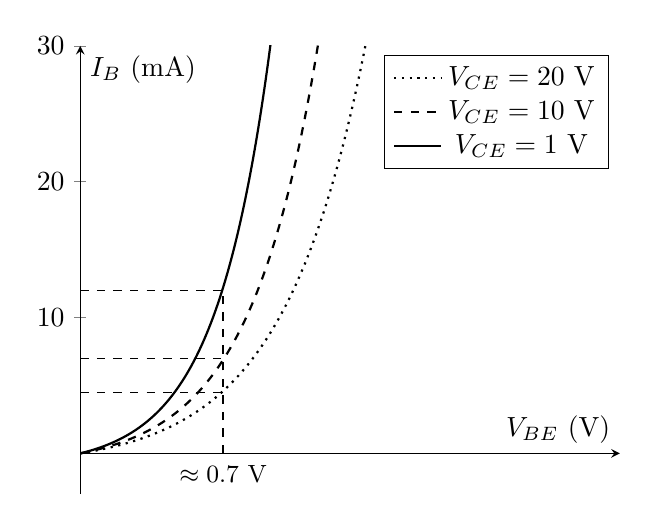
\begin{tikzpicture}
\begin{axis}[
    xlabel={$V_{BE}$ (V)},
    ylabel={$I_{B}$ (mA)},
    xmin=0, xmax=6.5,
    ymin=-3, ymax=30,
    axis lines=middle,
    xtick=\empty,
]

\addplot[
    domain=0:3.5,
    samples=200,
    dotted, thick
]
{(e^x-1)};
\addlegendentry{$V_{CE}=20$ V}

\addplot[
    domain=0:3.5,
    samples=200,
    dashed, thick
]
{(e^(1.2*x)-1)};
\addlegendentry{$V_{CE}=10$ V}

\addplot[
    domain=0:3.5,
    samples=200,
    thick
]
{(e^(1.5*x)-1)};
\addlegendentry{$V_{CE}=1$ V}

\node at (axis cs: 1.72, -1.5) {\small $\approx0.7$ V};
\draw[dashed] (axis cs: 1.72, 0)--(axis cs: 1.72, 12) (axis cs: 0, 12)--(axis cs: 1.72, 12) (axis cs: 0, 7)--(axis cs: 1.72, 7) (axis cs: 0, 4.5)--(axis cs: 1.72, 4.5);

\end{axis}
\end{tikzpicture}

\small \textit{Graph 1: Input characteristics curve for a BJT}
\end{center}
\item The graph is given.
\begin{center}
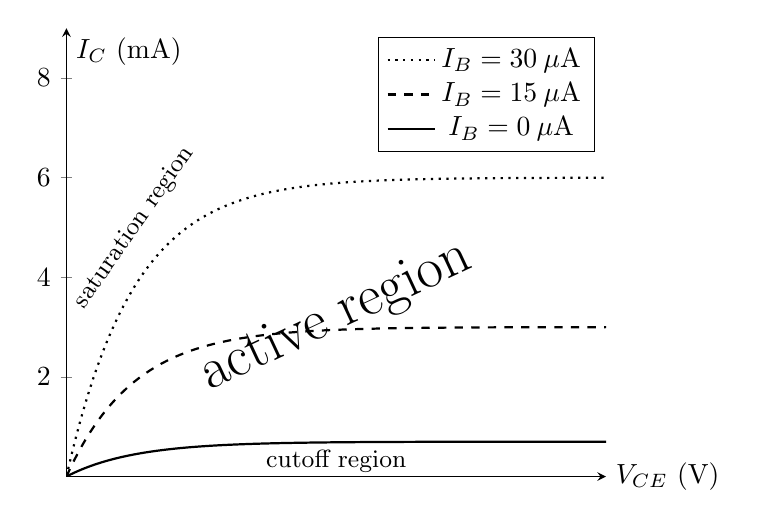
\begin{tikzpicture}
\begin{axis}[
    axis lines=center,
    xlabel={$V_{CE}$ (V)},
    xlabel style={at={(axis description cs:1,0)}, anchor=west},
    ylabel={$I_{C}$ (mA)},
    xmin=0, xmax=8,
    ymin=0, ymax=9,
    xtick=\empty,
]

\addplot[
    domain=0:8,
    samples=200,
    dotted, thick
]
{6*(1 - exp(-x))};
\addlegendentry{$I_B = 30\:\mu$A}

\addplot[
    domain=0:8,
    samples=200,
    dashed, thick
]
{3*(1 - exp(-x))};
\addlegendentry{$I_B = 15\:\mu$A}

\addplot[
    domain=0:8,
    samples=200,
    thick
]
{0.7-0.7*exp(-x))};
\addlegendentry{$I_B = 0\:\mu$A}

\node at (axis cs: 4, 0.3) {\small cutoff region};
\node[rotate=25] at (axis cs: 4, 3.2) {\huge active region};
\node[rotate=55] at (axis cs: 1, 5) {\small saturation region};

\end{axis}
\end{tikzpicture}

\small \textit{Graph 2: Output characteristics curve for a BJT}
\end{center}

\end{enumerate}

\textbf{Simulation}

\begin{enumerate}[leftmargin=*,label=\textbf{\arabic*.}]

\setcounter{enumi}{1}

\item The graph is given below.

\begin{minipage}{0.47\textwidth}
\begin{figure}[H]
    \centering
    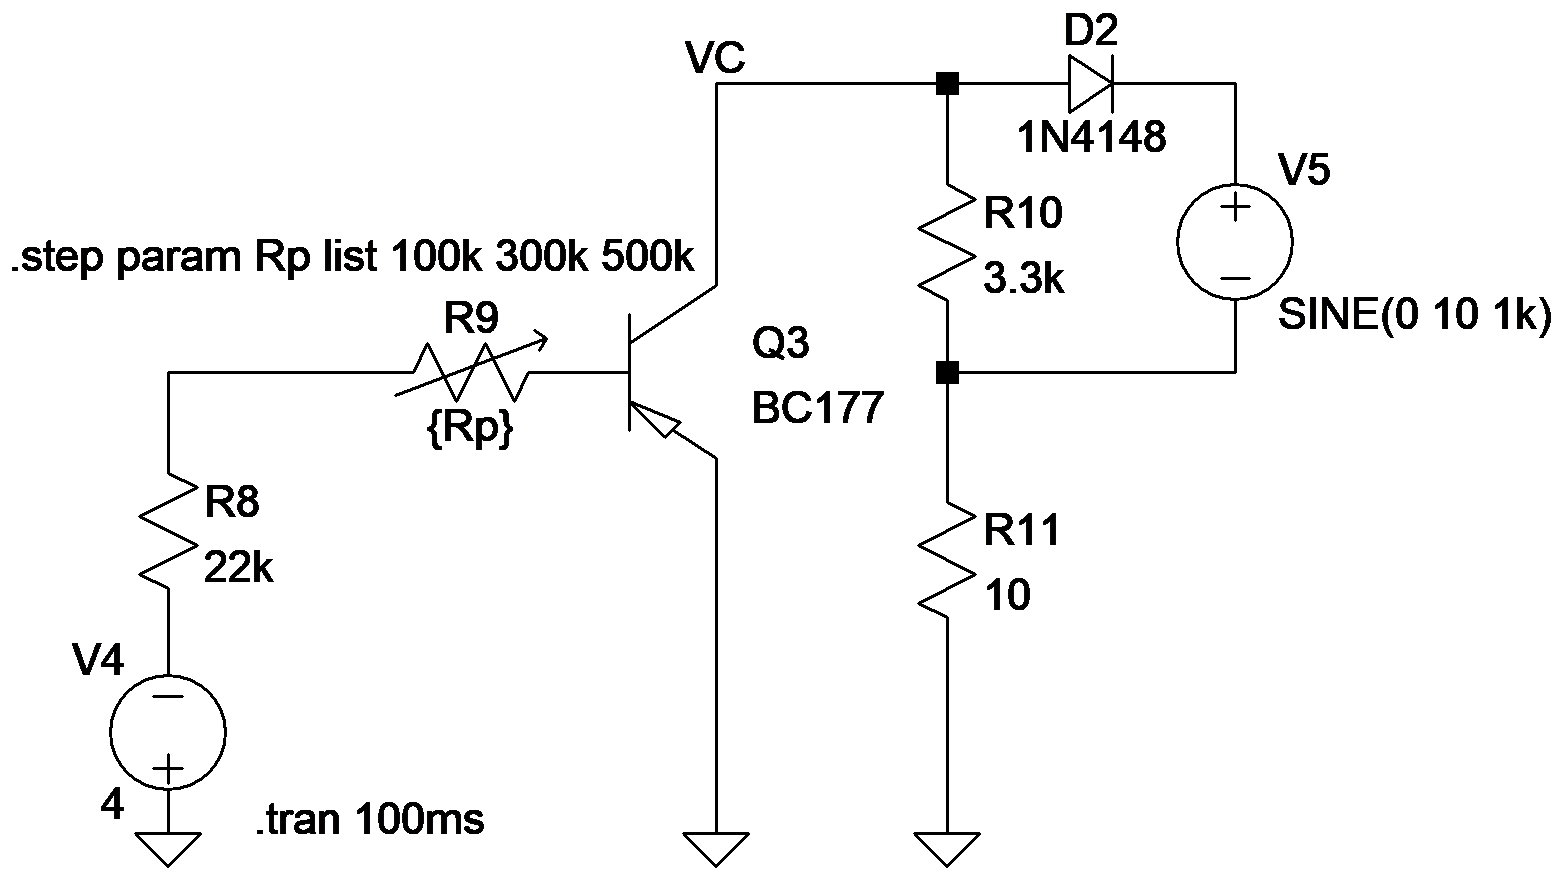
\includegraphics[width=1\linewidth]{c1_1.png}

    \small \textit{Figure 3: Figure 1 adjusted}
\end{figure}
\end{minipage}\hfill\begin{minipage}{0.49\textwidth}
\begin{figure}[H]
    \centering
    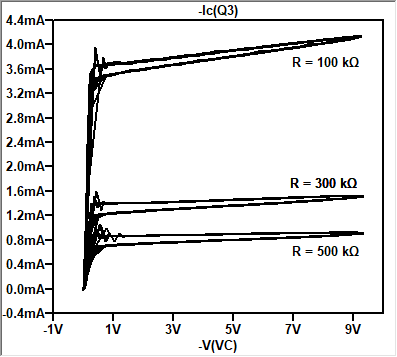
\includegraphics[width=0.9\linewidth]{LTspice_DneLKLXJWS.png}

    \small \textit{Graph 3: Output characteristics curve for Figure 3}
\end{figure}
\end{minipage}

\[I_C=-4.14 \text{ mA for } R=100 \text{ k}\Omega,\]
\[I_C=-1.51 \text{ mA for } R=300 \text{ k}\Omega,\]
\[I_C=-0.91 \text{ mA for } R=500 \text{ k}\Omega.\]

\item The graph is given below.

\begin{minipage}{0.47\textwidth}
\begin{figure}[H]
    \centering
    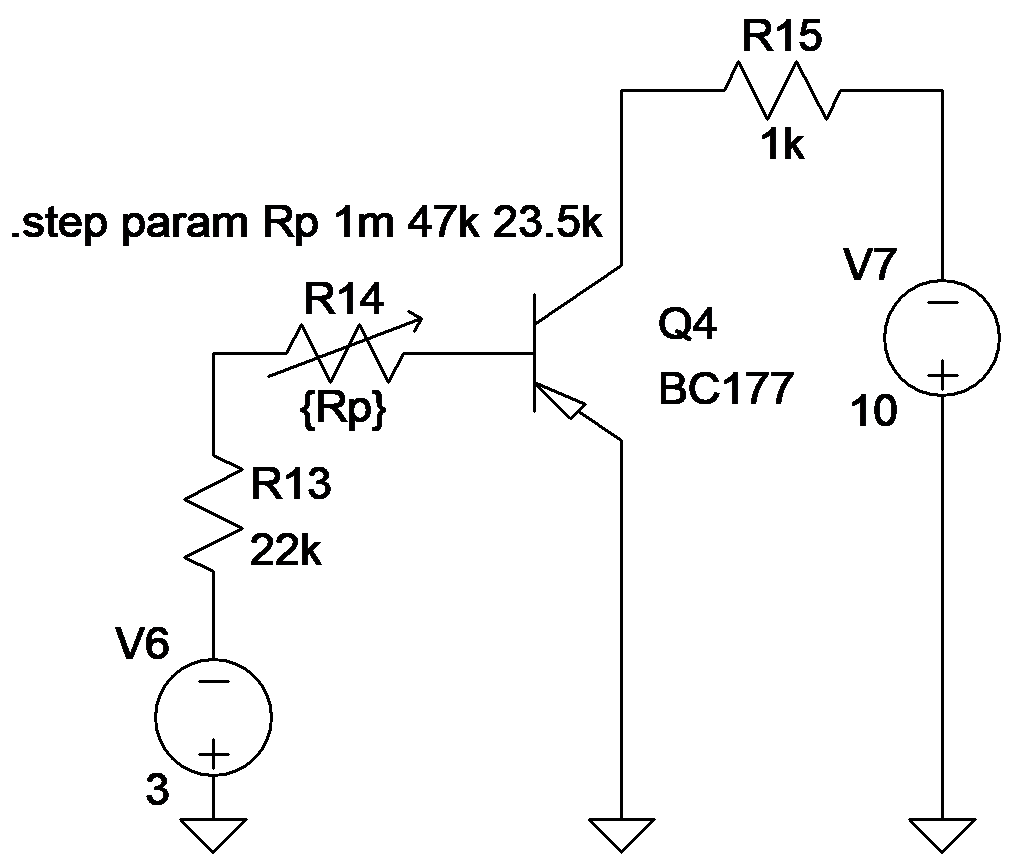
\includegraphics[width=1\linewidth]{c2_1.png}

    \small \textit{Figure 4: Figure 2 adjusted}
\end{figure}
\end{minipage}\hfill\begin{minipage}{0.49\textwidth}
\begin{figure}[H]
    \centering
    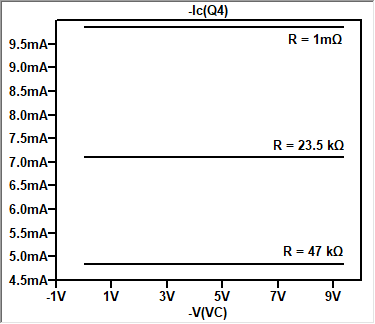
\includegraphics[width=0.9\linewidth]{LTspice_I9PkJwYNkZ.png}

    \small \textit{Graph 4: Output characteristics curve for Figure 4}
\end{figure}
\end{minipage}

\[I_C=-9.85 \text{ mA for } R=1 \text{ m}\Omega\approx0\:\Omega,\]
\[I_C=-7.10 \text{ mA for } R=23.5 \text{ k}\Omega,\]
\[I_C=-4.86 \text{ mA for } R=47 \text{ k}\Omega.\]

Base resistances:
\[R_{B}=0+22\text{ k}=22\text{ k}\Omega \text{ for }  I_C=-9.85 \text{ mA},
\]
\[R_{B}=23.5+22\text{ k}=45.5\text{ k}\Omega \text{ for }  I_C=-7.10 \text{ mA},\]
\[R_{B}=47+22\text{ k}=69\text{ k}\Omega \text{ for } I_C=-4.86 \text{ mA}.\]

\end{enumerate}

\end{document}